\documentclass[11pt]{article}
\usepackage[utf8]{inputenc}
\usepackage[T1]{fontenc}
\usepackage{amsmath}
\usepackage{amssymb}
\usepackage{tikz}
\usepackage{xcolor}
\usepackage[margin=1in]{geometry}

% Librerías de TikZ necesarias
\usetikzlibrary{matrix, positioning, arrows.meta, backgrounds, calc}

% Definición de colores basados en la imagen
\definecolor{titleblue}{HTML}{0D1B36} % Azul oscuro para el texto
\definecolor{rowcyan}{HTML}{9DF0ED}   % Celeste para la fila
\definecolor{colyellow}{HTML}{F9F097} % Amarillo para la columna
\definecolor{intgreen}{HTML}{8BEA84}  % Verde para la intersección

\begin{document}

\sffamily % Usar fuente sans-serif para asemejar el estilo de presentación
\color{titleblue} % Color base para el texto

% --- TÍTULO ---
{\LARGE \textbf{Definición Formal: El Arreglo}\\ \textbf{Bidimensional}}\\[1.5em]

% --- CONTENIDO PRINCIPAL ---
\noindent
\begin{minipage}[c]{0.45\textwidth}
    Una matriz $A$ es un arreglo de \\ $m \cdot n$ números reales.
    \vspace{0.5em}
    \begin{itemize}
        \item Tamaño: $m \text{ filas} \times n \text{ columnas}$.
        \item Notación: $A = (a_{ij})$
        \item Ubicación: $i$ indica la fila $(1\dots m)$\\ y $j$ la columna $(1\dots n)$.
    \end{itemize}
\end{minipage}%
\hfill
\begin{minipage}[c]{0.5\textwidth}
    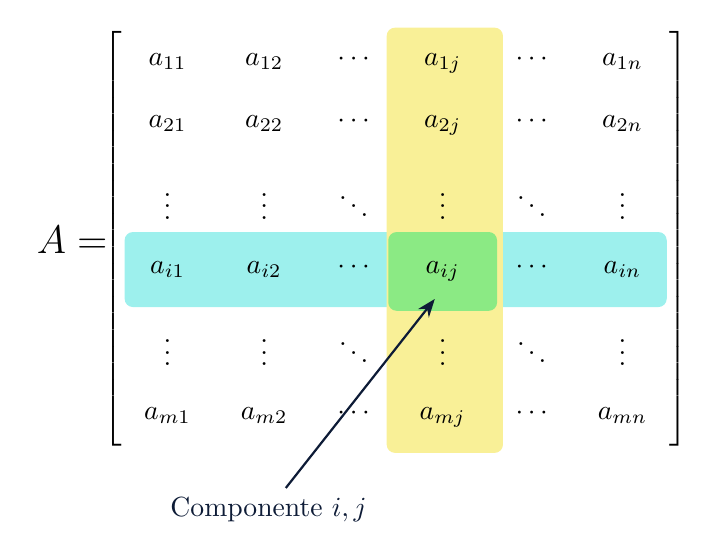
\begin{tikzpicture}[>=Stealth]
        % Etiqueta "A ="
        \node (A_label) at (-0.5, 0) {\Large $A = $};
        
        % Matriz con TikZ
        \matrix (M) [
            matrix of math nodes,
            left delimiter={[}, right delimiter={]},
            row sep=0.3cm, column sep=0.4cm,
            right=0.1cm of A_label
        ] {
            a_{11} & a_{12} & \cdots & a_{1j} & \cdots & a_{1n} \\
            a_{21} & a_{22} & \cdots & a_{2j} & \cdots & a_{2n} \\
            \vdots & \vdots & \ddots & \vdots & \ddots & \vdots \\
            a_{i1} & a_{i2} & \cdots & a_{ij} & \cdots & a_{in} \\
            \vdots & \vdots & \ddots & \vdots & \ddots & \vdots \\
            a_{m1} & a_{m2} & \cdots & a_{mj} & \cdots & a_{mn} \\
        };

        % Capa de fondo para los resaltados de color
        \begin{scope}[on background layer]
            % Resaltado de la Fila (Celeste)
            \fill[rowcyan, rounded corners=3pt] 
                ([xshift=-0.2cm, yshift=0.25cm]M-4-1.north west) 
                rectangle 
                ([xshift=0.2cm, yshift=-0.25cm]M-4-6.south east);
                
            % Resaltado de la Columna (Amarillo)
            \fill[colyellow, rounded corners=3pt] 
                ([xshift=-0.35cm, yshift=0.2cm]M-1-4.north west) 
                rectangle 
                ([xshift=0.35cm, yshift=-0.2cm]M-6-4.south east);
                
            % Resaltado de la Intersección (Verde)
            \fill[intgreen, rounded corners=3pt] 
                ([xshift=-0.35cm, yshift=0.25cm]M-4-4.north west) 
                rectangle 
                ([xshift=0.35cm, yshift=-0.25cm]M-4-4.south east);
        \end{scope}

        % Flecha y etiqueta inferior
        \node[titleblue, below left=2.5cm and 0.5cm of M-4-4] (text_comp) {Componente $i, j$};
        \draw[->, thick, titleblue] (text_comp) -- ([yshift=-0.1cm, xshift=-0.1cm]M-4-4.south);
        
    \end{tikzpicture}
\end{minipage}

\end{document}
